\documentclass[10pt,letterpaper]{article}
%\usepackage{times}
\usepackage[margin=1in,hmargin=1in]{geometry}
\usepackage{amsmath}
\usepackage{tikz,url}
\usepackage{amssymb}
\usepackage{fancyhdr}
\usetikzlibrary{matrix}
\usepackage{listings}
\usepackage{tabularx}
\usepackage{xcolor}
\usepackage{graphicx}
\usepackage{graphics}
\usepackage{titling}
\pagestyle{fancy}
\usepackage{float}
\usepackage{fancyvrb}
\usepackage{verbatim}
\usepackage{enumitem}
\usepackage{alltt}
\usepackage{pdfpages}
\usepackage{multicol}
%\restylefloat{table}

\fancyhead[LO]{STAT W4201 Advanced Data Analysis}
\fancyhead[RO]{HW 8}
\fancyhead[LE]{STAT W4201 Advanced Data Analysis}
\fancyhead[RE]{HW 8}
\title{\textbf {Homework 8}}
\author{{Qianbo Wang}\\{uni: qw2180}}
\date{}
\setlength{\droptitle}{-5em}
\setlength{\parindent}{0pt}
\makeatletter
\newcommand{\rmnum}[1]{\romannumeral #1}
\newcommand{\Rmnum}[1]{\expandafter\@slowromancap\romannumeral #1@}
\makeatother
\lstset{
language=R,
tabsize=4, 
%frame=shadowbox, 
commentstyle=\color{red!50!green!50!blue!50},
%rulesepcolor=\color{red!20!green!20!blue!20},
keywordstyle=\color{blue!90},
showstringspaces=false,
stringstyle=\ttfamily, 
keepspaces=true, 
breakindent=22pt, 
numbers=none,
stepnumber=1,
numberstyle=\tiny, 
numberstyle={\color[RGB]{0,192,192}\tiny} ,
numbersep=5pt,  
basicstyle=\footnotesize, 
showspaces=false, 
flexiblecolumns=true, 
comment=[l]{\#},
texcl=true,
escapeinside={\$$}{\^^M},
breaklines=true, 
breakautoindent=true,
breakindent=4em, 
aboveskip=1em, 
tabsize=2,
showstringspaces=false, 
backgroundcolor=\color[RGB]{244,244,244},   
fontadjust,
captionpos=t,
framextopmargin=2pt,framexbottommargin=2pt,abovecaptionskip=-3pt,belowcaptionskip=3pt,
extendedchars=false,columns=flexible
}

\RecustomVerbatimCommand{\VerbatimInput}{VerbatimInput}{fontsize=\footnotesize}
\begin{document}
\maketitle
\thispagestyle{fancy}
\vspace{-2em}

\section*{Problem 1}
\textbf{Reading Assignment: Ramsey and Schafer (2nd Ed), Chapter 22 (Log-Linear Regression for Poisson Counts)}

\section*{Problem 2}
\textbf{Consider the Valve characteristics data (Display 22.16, Ramsey and Schafer, 2nd Ed).}\\

Valve Failure in Nuclear Reactors. Display 22.16 shows characteristics and numbers of failures
observed in valve types from one pressurized water reactor. There are five explanatory factors:
\begin{enumerate}[leftmargin=0cm,itemindent=.5cm,labelwidth=\itemindent,labelsep=0cm,align=left]
\item[\textbullet] system (1 = containment, 2 = nuclear, 3 = power conversion, 4 = safety, 5 = process auxiliary);
\item[\textbullet] operator type (1 = air, 2 = solenoid, 3 = motor-driven, 4 = manual); 
\item[\textbullet] valve type (1 = ball, 2 = butterfly, 3 = diaphragm, 4 = gate, 5 = globe, 6 = directional control); 
\item[\textbullet] head size (1 = less than 2 inches, 2 = 2–10 inches, 3 = 10–30 inches); 
\item[\textbullet] operation mode (1 = normally closed, 2 = normally open). 
\end{enumerate}
The lengths of observation periods are quite different, as indicated in the last column, time. Using an offset for log of observation time, identify the factors associated with large numbers
of valve failures.
\begin{enumerate}[leftmargin=0cm,itemindent=.5cm,labelwidth=\itemindent,labelsep=0cm,align=left]
\item[\textbf{(a).} ] \textbf{Do Problem Number 24, Page 667, using the R function glm.}

First, use all of the variables to fit a log-linear poisson regression model with log(time) as offset. And the result is as follows:
\begin{center}
Log-linear Poisson Regression 
\VerbatimInput{glmpoisson.txt}
\end{center}
So the model is:
\begin{equation*}
\begin{split}
log(Failures) = -3.77 & + 0.92System2+1.02System3+1.22System4+0.33System5\\
& + 0.70Operator2-1.19Operator3-2.47Operator4\\
& + 0.19Valve2+0.61Valve3+2.96Valve4+1.79Valve5+1.01Valve6\\
& - 0.01Size2+1.1Size3\\
& - 0.21Mode2
\end{split}
\end{equation*}


And since there are several coefficients not significant, this means that these corresponding variables are not associated with Failures. \\

\item[\textbf{(b).} ] \textbf{Interpret the estimated parameters.}

There are total 16 parameters here in the model. $\beta_0$ as the intercept, i.e., when System, Operator, Valve, Size and Mode all equal 1, the $ =e^{-3.77}$. $\beta_1-\beta_4$, as the coefficients of 4 different System levels 2-5, respectively. $\beta_5-\beta_7$, as the coefficients of 3 different Operator levels 2-4, respectively. $\beta_8-\beta_{12}$, as the coefficients of 5 different Valve levels 2-6, respectively. $\beta_{13}-\beta_{14}$, as the coefficients of 5 different levels Size 2-3, respectively and $\beta_{15}$, as the coefficient of Mode level 2.
\begin{enumerate}[leftmargin=0cm,itemindent=.5cm,labelwidth=\itemindent,labelsep=0cm,align=left]
\item[\textbullet] System

When other explanatory variables are fixed, then System 2 will cause $e^{0.92}=2.509$ times as many Failures as System 1, and similarly System 3 will cause $e^{1.02}=2.773$ times as many Failures as System 1, System 4 will cause $e^{1.22}=3.387$ times as many Failures as System 1. System 5 will cause $e^{0.33}=1.391$ times as many Failures as System 1. And since under 0.05 significance level, the coefficients of System 2 and System 5 are not significant, then this means that System 2 and System 5 are not different from System 1 in the sense of Large number of Failures.

\item[\textbullet] Operator

When other explanatory variables are fixed, then Operator 2 will cause $e^{0.70}=2.014$ times as many Failures as Operator 1, and similarly Operator 3 will cause $e^{-1.19}=0.304$ times as many Failures as System 1, Operator 4 will cause $e^{-2.47}=0.085$ times as many Failures as Operator 1.  And since under 0.05 significance level, the coefficient of Operator 2 is not significant, then this means that Operator 2 is not different from System 1 in the sense of Large number of Failures.

\item[\textbullet] Valve

When other explanatory variables are fixed, then Valve 2 will cause $e^{0.19}=1.20$ times as many Failures as Valve 1, and similarly Valve 3 will cause $e^{0.61}=1.84$ times as many Failures as Valve 1, Valve 4 will cause $e^{2.96}=19.298$ times as many Failures as Valve 1, Valve 5 will cause $e^{1.79}=5.990$ times as many Failures as Valve 1, Valve 6 will cause $e^{1.01}=2.746$ times as many Failures as Valve 1. And since under 0.05 significance level, the coefficients of Valve 2, Valve 3 and Valve 6 are not significant, then this means that Valve 2, Valve 3 and Valve 6 are not different from System 1 in the sense of Large number of Failures.

\item[\textbullet] Size

When other explanatory variables are fixed, then Size 2 will cause $e^{-0.01}=0.990$ times as many Failures as Size 1, and similarly Size 3 will cause $e^{1.61}=5.002$ times as many Failures as Size 1.  And since under 0.05 significance level, the coefficient of Size 2 is not significant, then this means that Size 2 is not different from Size 1 in the sense of Large number of Failures.

\item[\textbullet] Mode

When other explanatory variables are fixed, then Mode 2 will cause $e^{-0.20}=0.819$ times as many Failures as Mode 1. And since under 0.05 significance level, the coefficient of Mode 2 is not significant, then this means that Mode 2 is not different from Mode 1 in the sense of Large number of Failures.
\end{enumerate}
\item[\textbf{(c).} ] \textbf{Assess the goodness of fit of the model}

\begin{center}
\small{Goodness of fit test Result}
\VerbatimInput{glmgoodness.txt}
\end{center}
From result of Deviance Goodness of Fit Test, the p-value is approximate to 1 which means that either the model is adequate or that insufficient data are available to detect inadequacies.\\

And the Chi-square Anova Table of log-linear regression result is as follows:
\begin{center}
\small{Log-Linear ANOVA Table}
\VerbatimInput{glmchisq.txt}
\end{center}
Since under 0.05 significance level, the Operator and Mode of explanatory variables are not significant. Then we can conclude that they are not strongly associated with Failures. 
\end{enumerate}

\section*{Problem 3}
\textbf{Repeat 2(a) using the glmnet package and comment on the results.}\\

Use cross validation and log linear poisson regression on the data. \\
The following plot shows the best lambda:
\begin{center}
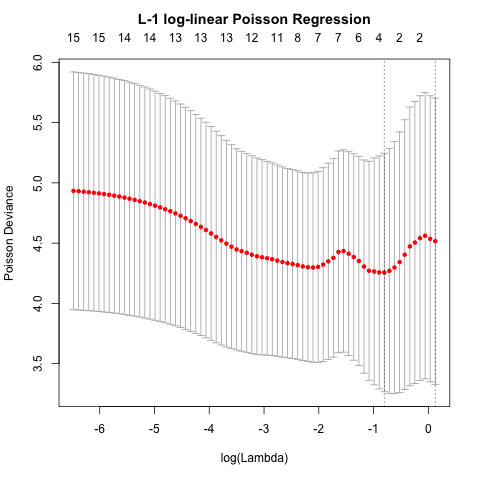
\includegraphics[scale=0.7]{glmpoisson_l1_cv}
\end{center}
So the best lambda is 0.1644754 and the corresponding coefficients are:
\begin{center}
\small{Coefficients of log-linear poisson regression with lasso}
\verbatiminput{glmpoisson_l1_cv.txt}
\end{center}
And the model is:
\[log(Failures)=-1.4249+0.7310Valve4+0.5531Size3\]

\textbf{Compare the results:}\\

Since from the two models we can find that, only Valve 4 and Size 3 are included in the model. Then this means only Valve 4 and Size 3 have significant effect on Failures. And compare the two models, we can find that these two models are quite different. And using Lasso with cross validation really depends on the seed because it depends on the training dataset. And lasso will reduce many variables, whereas, regular log-linear regression won't.


\newpage
\textbf{R Code:}
\begin{lstlisting}[language=R]
rm(list=ls())
library(Sleuth2)
data(ex2224)
Nuclear<-ex2224
levels(Nuclear$System)<-c("containment","nuclear","power conversion","safety","process auxiliary")
levels(Nuclear$Operator)<-c("air","solenoid","motor-driven","manual")
levels(Nuclear$Valve)<-c("ball","butterfly","diaphragm","gate","globe","directional control")
levels(Nuclear$Size)<-c("<2","2-10","10-30")
levels(Nuclear$Mode)<-c("closed","open")
for (names in names(Nuclear)){
  if (class(Nuclear[[names]])!="numeric"){
    Nuclear[[names]]<-as.factor(as.numeric(Nuclear[[names]]))
  }
}

#loglinear poisson regression 
glmpoisson<-glm(Failures~System+Operator+Valve+Size+Mode,offset=log(Time),data=Nuclear,family="poisson")
summary(glmpoisson)

sink('/Users/raymond/Drive/STAT W4201/HW8/glmpoisson.txt')
glmpoisson
summary(glmpoisson)
sink()

# goodness of fit test
Goodness_of_Fit<-cbind(res.deviance = sprintf("%.8f",glmpoisson$deviance),df = glmpoisson$df.residual, p.value = sprintf("%.8f",(1-pchisq(glmpoisson$deviance,glmpoisson$df.residual,lower.tail = FALSE))))

sink("/Users/raymond/Drive/STAT W4201/HW8/glmgoodness.txt")
cat("Goodness of Fit Test \n \n")
write.table(Goodness_of_Fit,row.names = FALSE,quote = FALSE,sep="   ")
sink()

sink("/Users/raymond/Drive/STAT W4201/HW8/glmchisq.txt")
anova(glmpoisson,test="Chisq")
sink()

#lasso log linear poisson regression
#data matrix transformation of dummy variables
library(glmnet)

NuclearData<-subset(Nuclear,select=c("Failures","Time"))
for (names in names(Nuclear)[1:5]){
  for (factor in levels(Nuclear[[names]])[-1]){
    NuclearData[[paste(names,factor,sep="")]]<-as.numeric(Nuclear[[names]]==factor)
  }
}
NuclearMat<-as.matrix(NuclearData[,-c(1,2)])
set.seed(123)
glmpoisson_l1<-glmnet(NuclearMat,NuclearData$Failures,offset=log(NuclearData$Time),family="poisson")
glmpoisson_l1_cv<-cv.glmnet(NuclearMat,NuclearData$Failures,offset=log(NuclearData$Time),family="poisson")

#plot the best lambda
png(filename = "/Users/raymond/Drive/STAT W4201/HW8/glmpoisson_l1_cv.png")
plot(glmpoisson_l1_cv)
title(main = "L-1 log-linear Poisson Regression", line = 2.5)
dev.off()

#get model coefficients
lambda<-glmpoisson_l1_cv$lambda.min
model<-glmpoisson_l1_cv$glmnet.fit
coeff<-coef(model,lambda)
sink('/Users/raymond/Drive/STAT W4201/HW8/glmpoisson_l1_cv.txt')
coeff
sink()
\end{lstlisting}
\end{document}